\documentclass{beamer}
\usepackage[utf8]{inputenc}
\usepackage{graphicx}
\usetheme{Montpellier}
%\usepackage{geometry}
%\geometry{top=2cm, bottom=2cm, left=2cm, right=2cm}
%\setbeamertemplate{footline}[frame number]


\title{}
\title{Présentation Backlog et Sprint 1 \\ Scrum Project Manager} 
\author{Fraj Saber, Jawhar Youssef, Laulan Antoine, Moudache Salim}
\institute{Université de Bordeaux}
\date{Année 2015/2016}

\begin{document}





%\AtBeginSection[]
%{
%    \begin{frame}
%        \frametitle{Plan}
%        \tableofcontents
%   \end{frame}
%}

%\AtBeginSubsection[]
%{
%    \begin{frame}
%        \frametitle{Plan}
%       \tableofcontents[currentsection, currentsubsection]
%   \end{frame}
%}

\begin{frame}
    \titlepage
\end{frame}



\section{Backlog}

\begin{frame}{Backlog}
	\begin{center}
        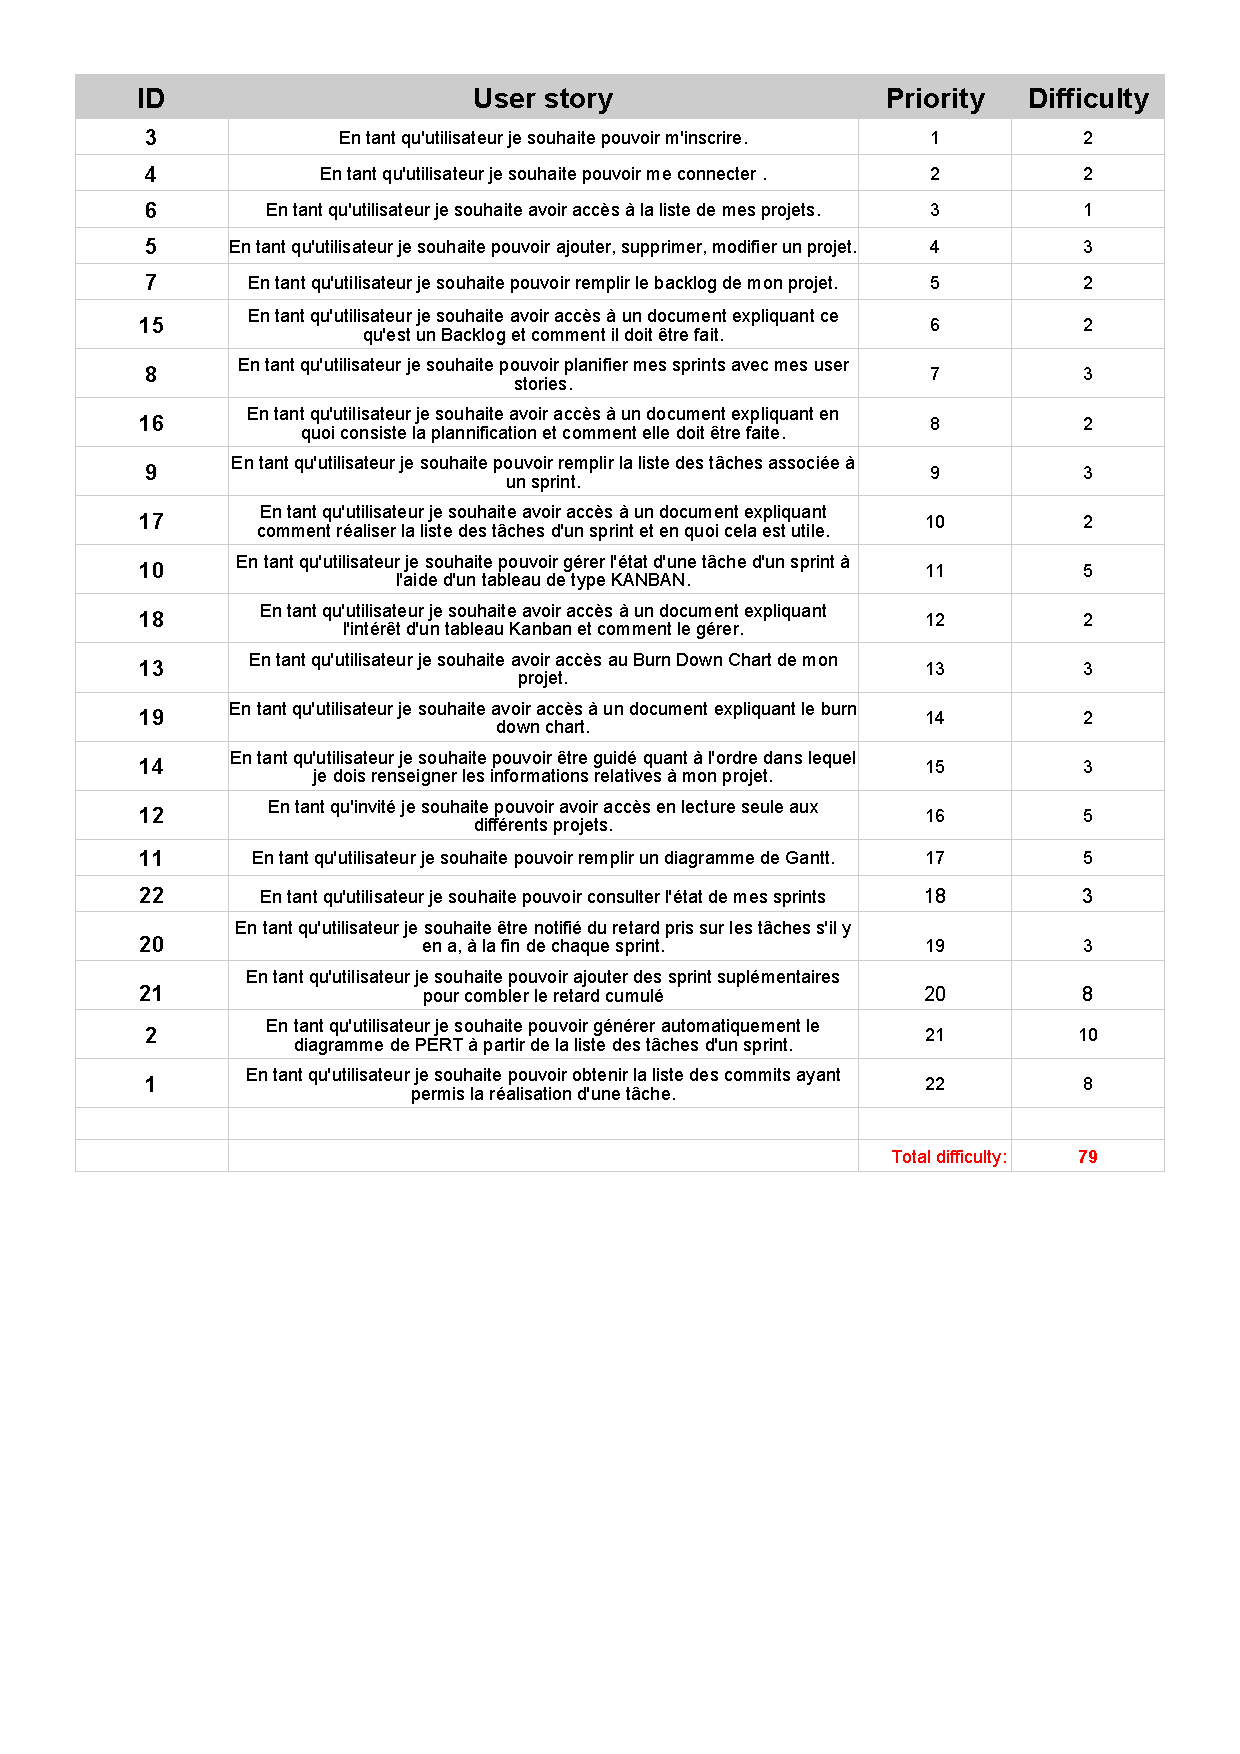
\includegraphics[scale=0.35]{BacklogPriority.pdf}
        \end{center}
\end{frame}

\section{Planning}

\begin{frame}{Planning}
	\begin{center}
        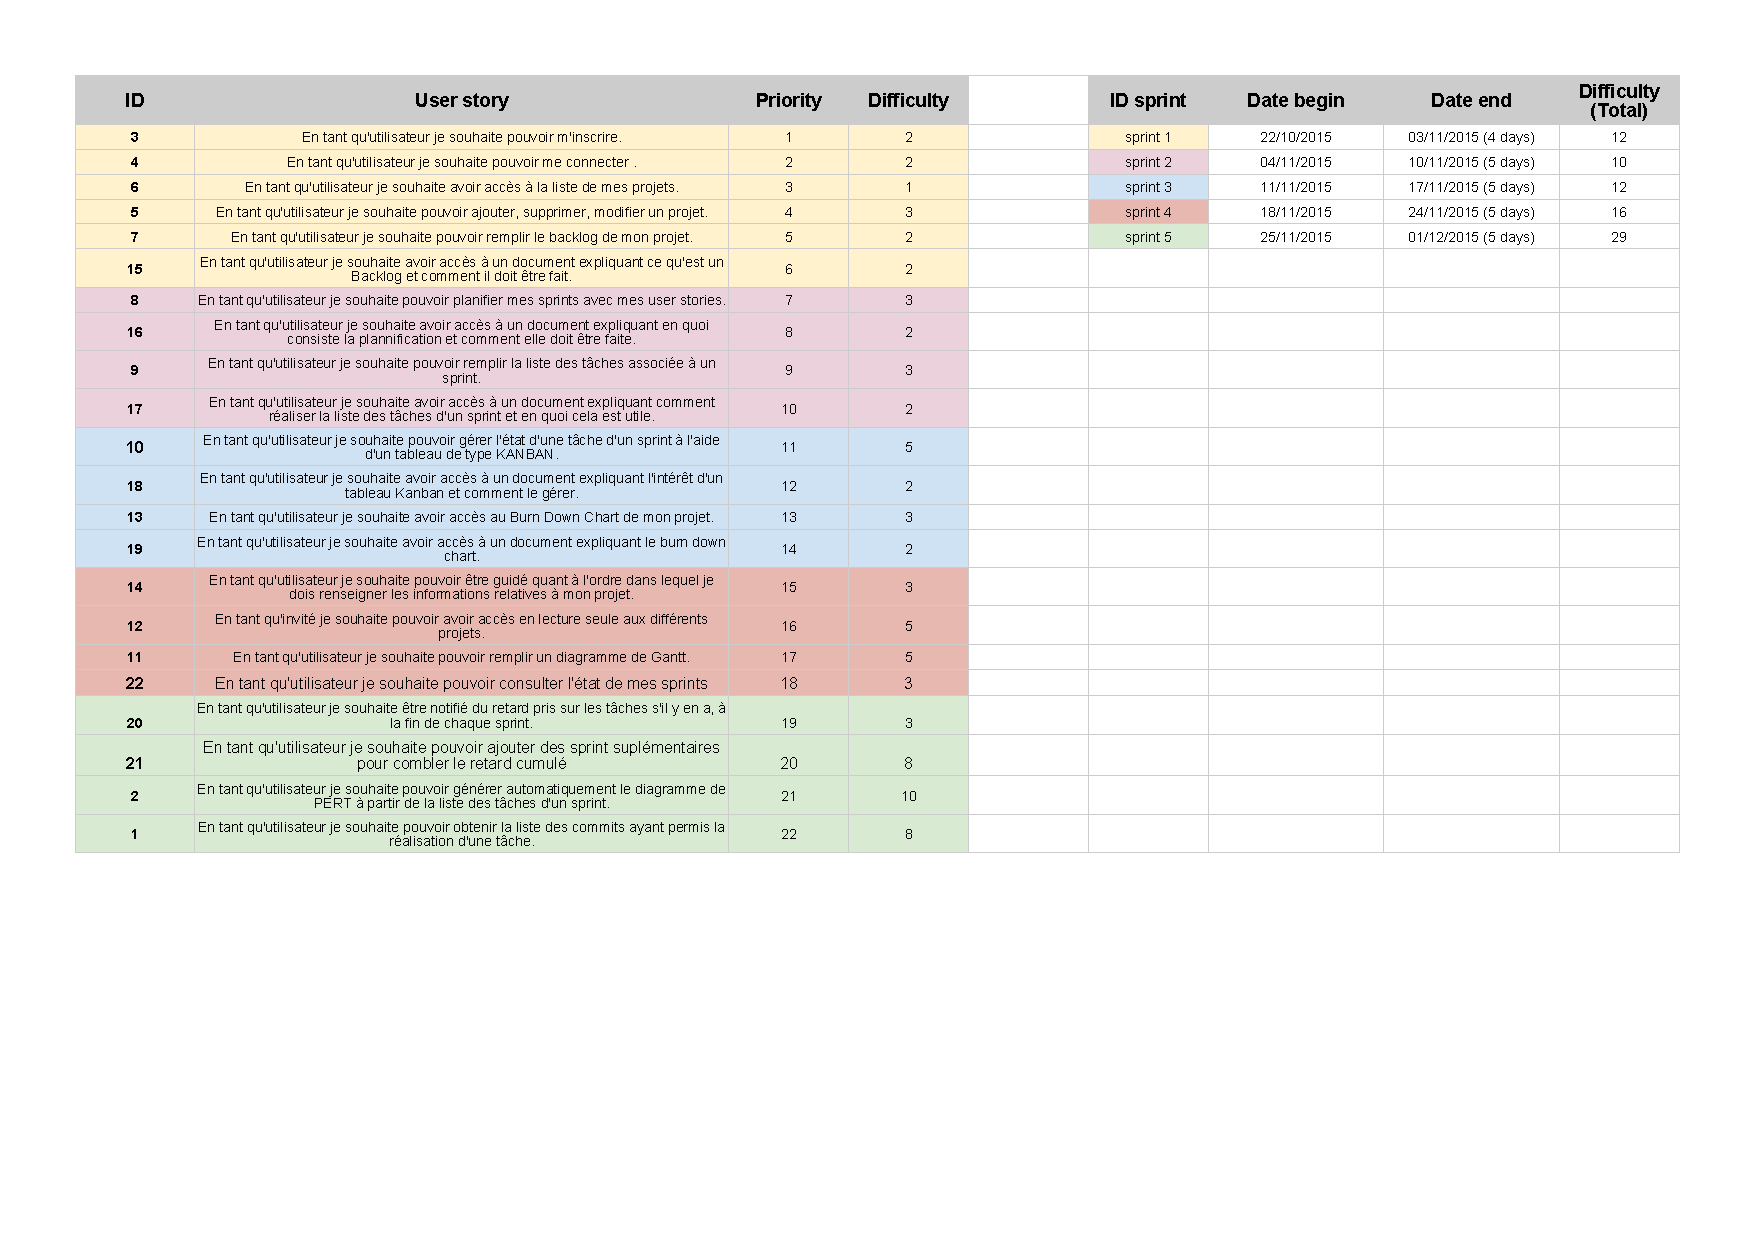
\includegraphics[scale=0.4]{Planning.pdf}
        \end{center}
\end{frame}

\section{Sprint 1}

\begin{frame}{Sprint 1}
	\begin{center}
        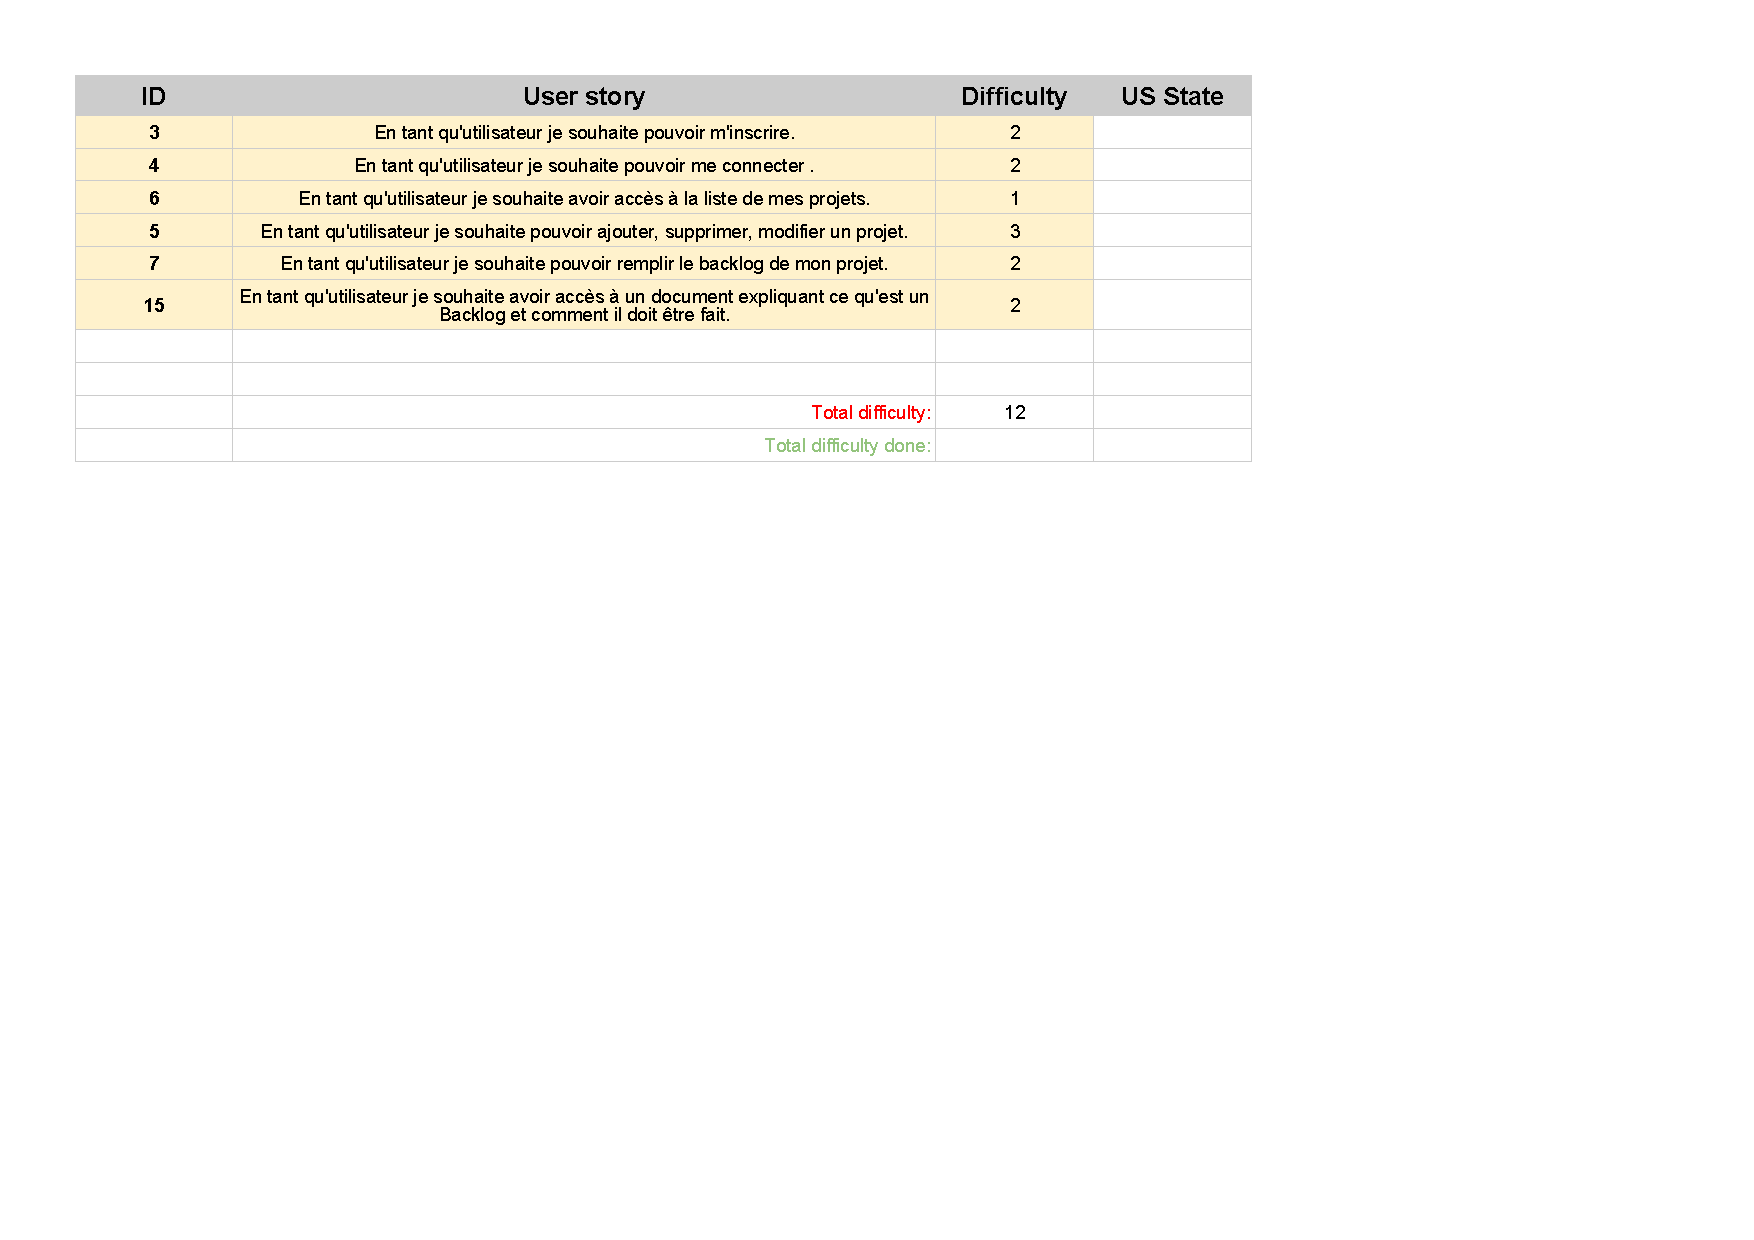
\includegraphics[scale=0.5]{Sprint1.pdf}
        \end{center}
\end{frame}

\subsection{Tasks List}

\begin{frame}{Tasks List}
	\begin{center}
        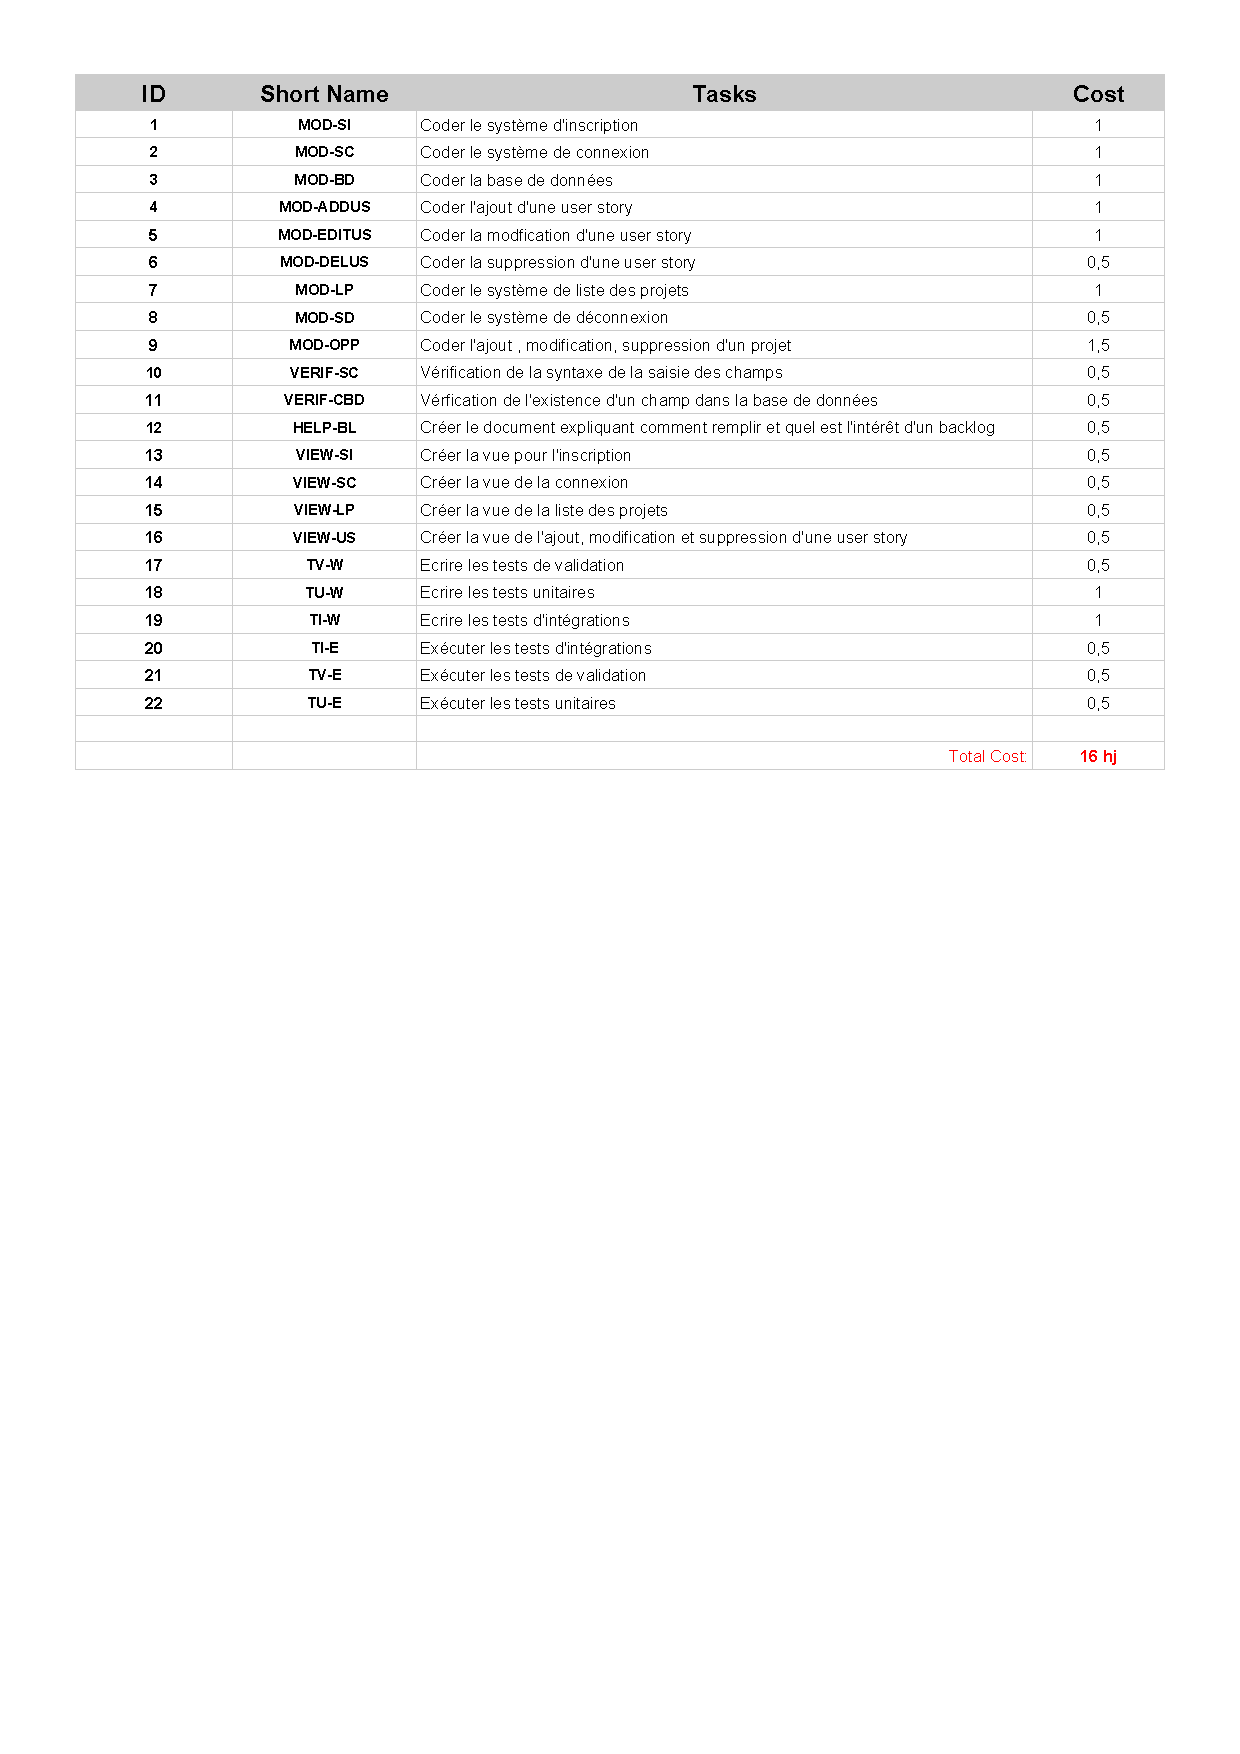
\includegraphics[scale=0.5]{TasksList.pdf}
        \end{center}
\end{frame}

\subsection{Pert Diagram}

\begin{frame}{Pert Diagram}
	\begin{center}
        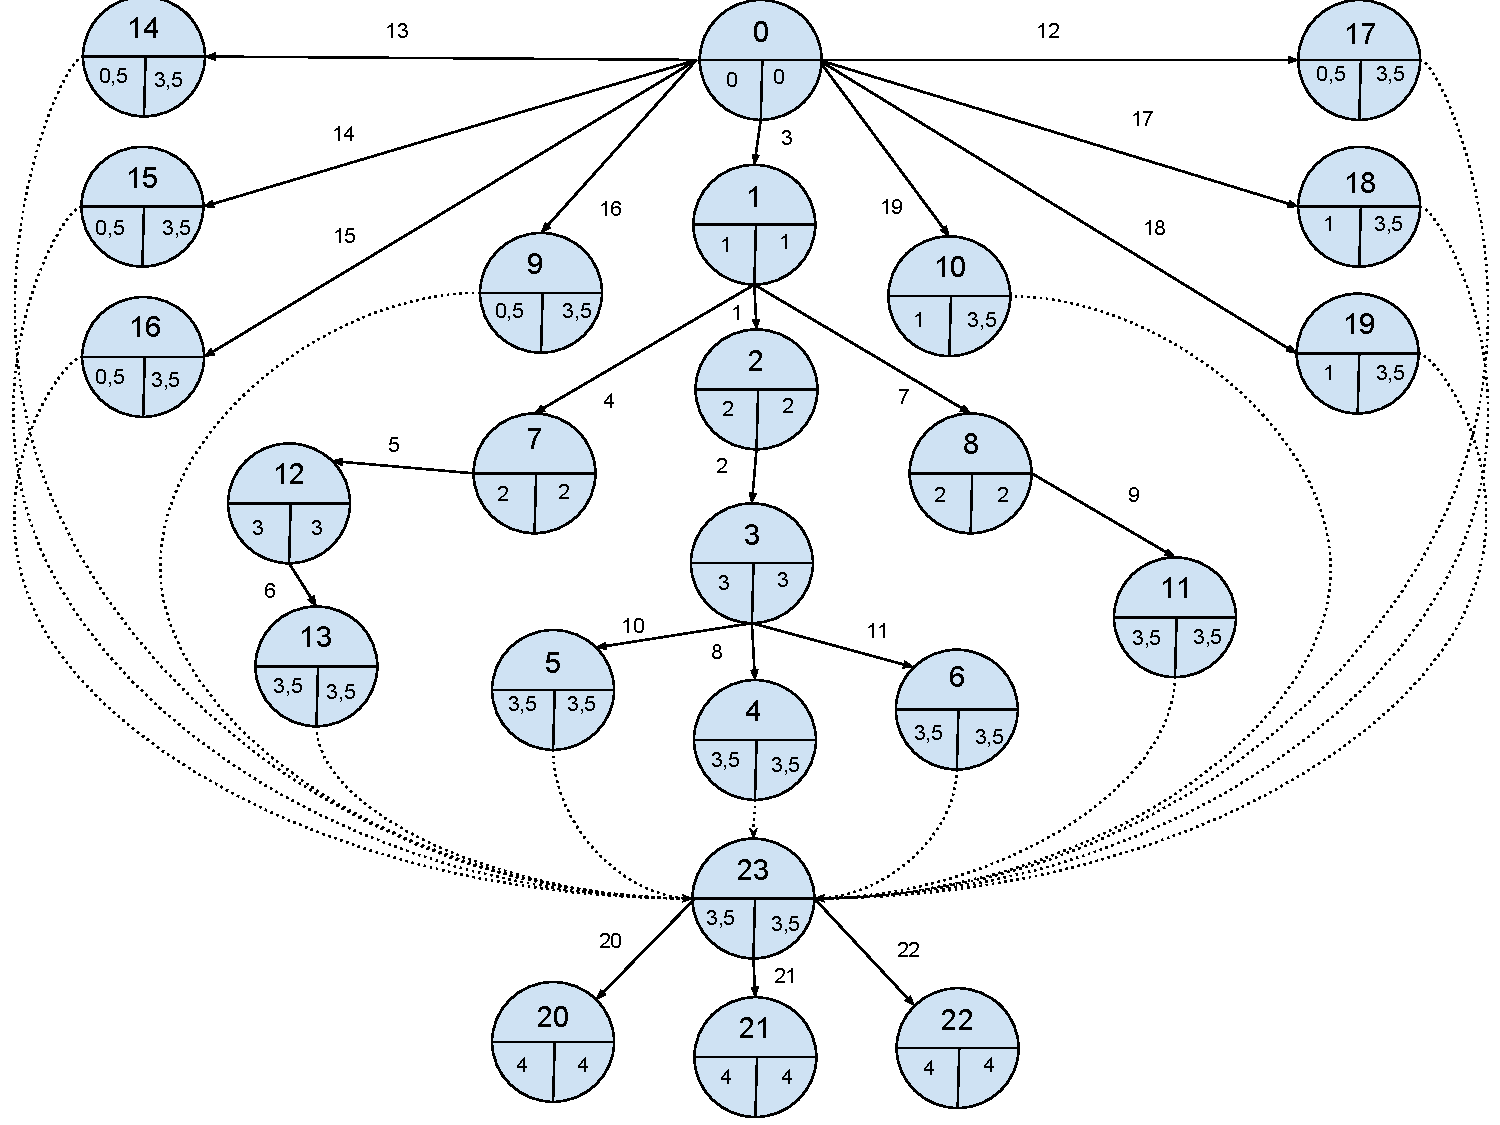
\includegraphics[scale=0.32]{Pert-Sprint1.pdf}
        \end{center}
\end{frame}


\subsection{Gantt Diagram}

\begin{frame}{Gantt Diagram}
	\begin{center}
        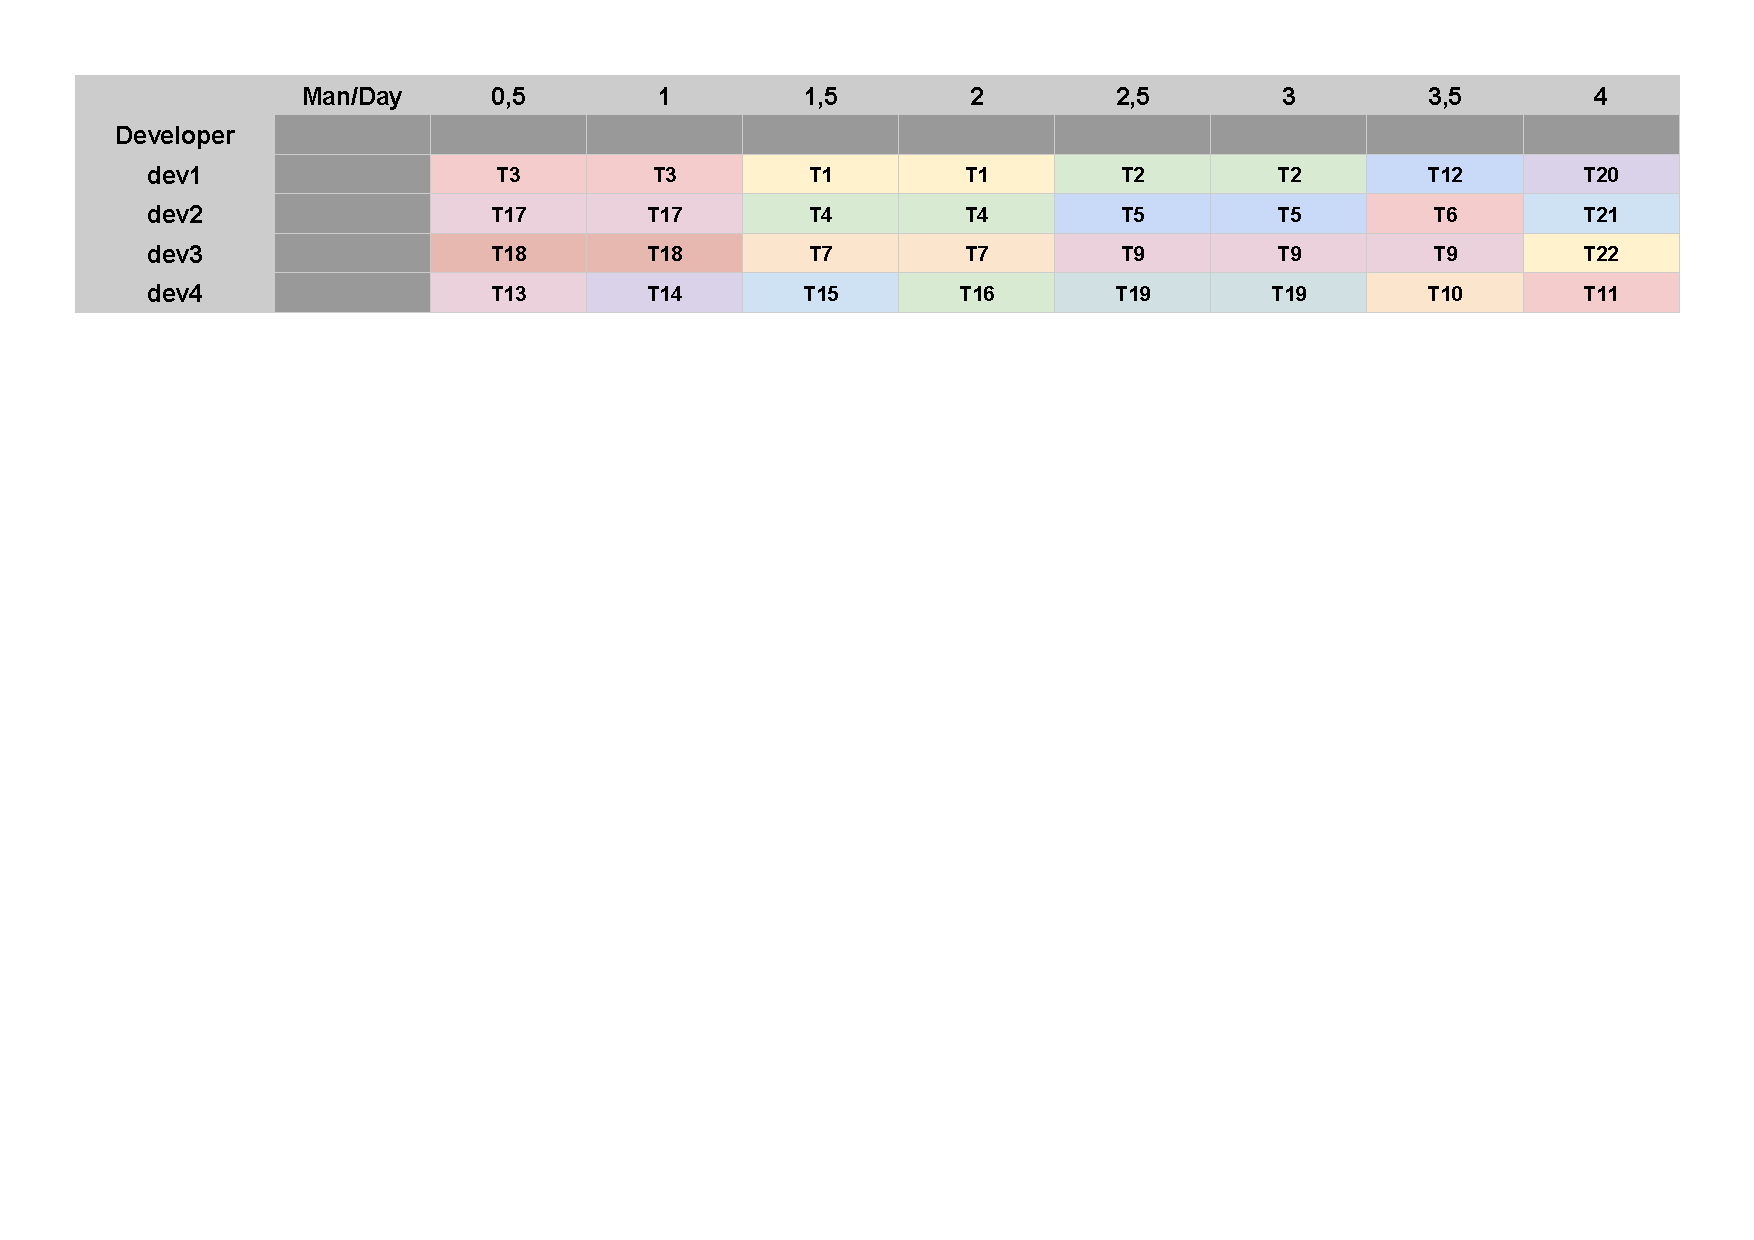
\includegraphics[scale=0.4]{Gantt1.pdf}
        \end{center}
\end{frame}

\subsection{Kanban}

\begin{frame}{First Kanban}
	\begin{center}
        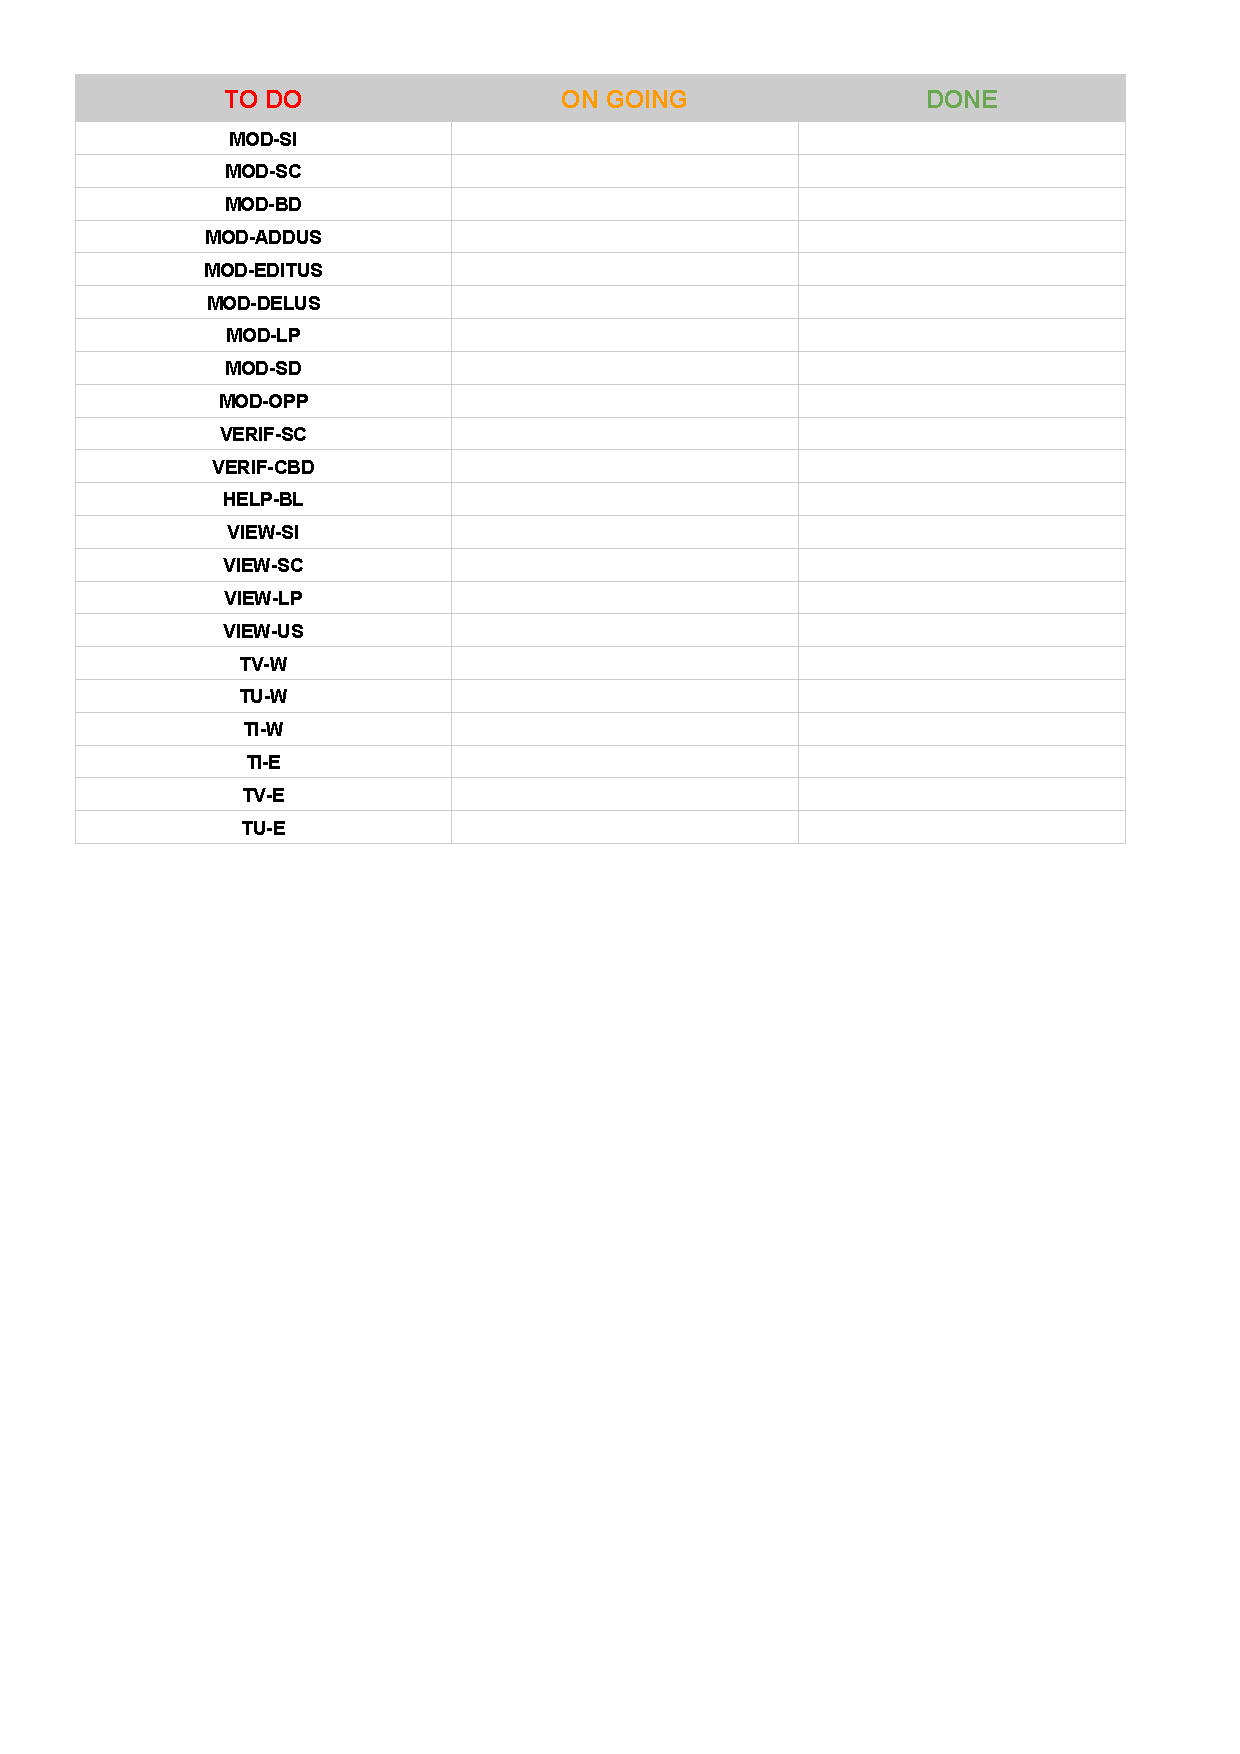
\includegraphics[scale=0.45]{Kanban1.pdf}
        \end{center}
\end{frame}




%%\begin{frame}{Contexte}
%%	\begin{center}
%%        \includegraphics[scale=0.13]{}
%%\end{frame}
%%
%%
%%\begin{frame}{Domaine}
%%	\begin{center}
%%        \includegraphics[scale=0.13]{}
%%    \end{center}
%%
%%	
%%\end{frame}
%%
%%
%%
%%\subsection{État de l'art}
%%
%%\begin{frame}{Télécommande Android}
%%	\begin{figure}
%%
%%	\begin{center}
%%        \includegraphics[scale=0.20]{}
%%        \caption{Denon Remote app \label{Figure 1}}
%%    \end{center}
%%
%%	\end{figure}
%%\end{frame}
%%
%%\begin{frame}{Analyse de données}
%%	\begin{figure}
%%	\begin{center}
%%        \includegraphics[scale=0.35]{}
%%        \caption{Kmeans \label{Figure 1}}
%%    \end{center}
%%    \end{figure}
%%\end{frame}
%%
%%
%%
%%
%%
%%
%%
%%\begin{frame}{Application : écoute et analyse}
%%    \begin{center}
%%    \setlength{\fboxsep}{2mm}
%%    \begin{tabular}{c c c c c}
%%        \fbox{\parbox{2.5cm}{\begin{center}Écoute de l'environnement\end{center}}} &
%%        $\longrightarrow$ &
%%        \fbox{\parbox{1.5cm}{\begin{center}Analyse des données\end{center}}} &
%%         $\longrightarrow$ &
%%         \fbox{Événements} \\
%%    \end{tabular}
%%
%%    \end{center}
%%
%%    \begin{tabular}{l p{6cm}l}
%%        \hline
%%        Écoute de l'environnement : & les capteurs font des mesures de quantités physiques de l'environnement. \\
%%        \hline
%%        Analyse des données : & utilisation d'algorithmes pour détecter des variations sur les mesures et en déduire
%%                                 des actions effectuées par l'utilisateur. \\
%%        \hline
%%        Événements : & résultats des analyses, l'utilisateur a-t-il provoqué une modification de l'environnement ? \\
%%    \end{tabular}
%%\end{frame}
%%
%%\begin{frame}{Application : Interface Homme Machine}
%%
%%    \begin{center}
%%        \includegraphics[scale=0.13]{}
%%    \end{center}
%%
%%\end{frame}
%%
%%
%%
%%
%%
%%\subsection{Fonctionnalités implémentées}
%%
%%\begin{frame}{Fonctionnalités implémentées}
%%	\begin{center}
%%	\begin{tabular}{c}
%%	      \includegraphics[scale=0.10]{} \\
%%	\end{tabular}
%%	\end{center}
%%
%%\end{frame}
%%
%%
%%\begin{frame}{Connexion}
%%	\begin{center}
%%	\begin{tabular}{c c}
%%		\includegraphics[scale=0.11]{} &
%%    	\includegraphics[scale=0.11]{} \\
%%      	\multicolumn{2}{c}{\includegraphics[scale=0.30]{}}
%%	\end{tabular}
%%	\end{center}
%%
%%\end{frame}
%%
%%\begin{frame}{Capteurs}
%%
%%	\begin{center}
%%	\begin{tabular}{c c c}
%%	 \includegraphics[scale=0.11]{} &
%%	 \includegraphics[scale=0.11]{} &
%%	 \includegraphics[scale=0.11]{} \\
%%	\end{tabular}
%%	\end{center}
%%
%%
%%\end{frame}


\end{document}
